\setcounter{page}{1}
\section*{Einleitung}
Die in den 1980er Jahren entwickelte Rasterkraftmikroskopie ist ein hochauflösendes Mikroskopieverfahren, welches auf der Wechselwirkung einer dünnnen Spitze mit der Oberfläche der betrachteten Probe beruht. Die Oberfläche der Probe wird dabei mithilfe der Spitze abgerastert, sodass ein dreidimensionales Abbild der Probe, aus der lateralen und vertikalen Position der Spitze erzeugt wird. Die Rasterkraftmikroskopie ist mit einer Auflösung von bis zu $\SI{0,1}{\pico\meter}$ das bislang hochauflösendste Strukturanalyseverfahren. Im Gegensatz zu anderen Mikroskopieverfahren ist es mit einem Rasterkraftmikroskop (AFM\footnote{Aus dem Englischen für \textbf{A}tomic \textbf{F}orce \textbf{M}icroscopy}) außerdem möglich, Messungen an nichtleitenden Proben vorzunehmen, sowie Messungen bei Normalbedingungen und in Flüssigkeiten durchzuführen. Neben der Analyse der Oberflächenstruktur, ist es zusätzlich möglich verschiedene mechanische Eigenschaften der Oberfläche wie zum Beispiel den Elastizitätsmodul oder die wirkende Adhäsionskraft zu messen. \\
\\
Ziel des vorliegenden Versuchs ist die Vermessung einer periodischen Mikrosturkturprobe und der Speicherpits einer CD und DVD mit dem AFM im \textit{constant-force} Modus\footnote{siehe \autoref{subsec:messmodi}}. Außerdem werden für die Materialien Edelstahl, Teflon und Kohlenstoff (in Form von DLC \footnote{Aus dem Englischen für \textbf{D}iamond \textbf{L}ike \textbf{C}arbon}) Kraftabstandskurven aufgenommen, um den Elastizitätsmodul, die Adhäsionskraft und die Federkonstante des Cantilevers\footnote{siehe \autoref{subsec:afmfunk}} zu bestimmen.
\newpage
\section{Theoretische Grundlagen}
Im Folgenden werden die für die Rasterkraftmikroskopie nötigen theoretischen und experimentellen Grundlagen anhand von Quelle \cite{Voigt} erläutert.
\subsection{Wirkende Kräfte zwischen Probe und Spitze}
Die zwischen Probe und Spitze wirkenden Kräfte können in lang- und kurzreichweitige, sowie abstoßende und anziehende Kräfte unterteilt werden.\\
Die für die Anziehung dominierende Kraft ist die London-Dispersionskraft (kurz LDK), die einen Teil der zwischen den Atomen wirkenden Van-der-Waals Kräfte ausmacht. Die LDK zählt zu den langreichweitigen Kräften und basiert auf der anziehenden Wechselwirkung spontan induzierter elektrischer Dipole in neutralen Atomen und Molekülen. Die Dipole entstehen durch Fluktuation der quantenmechanisch zu beschreibenden Ladungsdichteverteilungen der Elektronen. Das Potential zur LDK ist proportional zur inversen sechsten Potenz des Abstandes der betrachteten Wechselwirkungspartner und kann Näherungsweise als isotrop und additiv beschrieben werden.
Für die Berechnung der wirkenden LDK zwischen Spitze und Pobe müssen aufgrund der langen Reichweite der Kraft auch die durch die Atome im Volumen der Spitze induzierten Kräfte berücksichtigt werden.
Insgesamt lässt sich die London-Dispersionskraft durch
\begin{equation}
  F_{\text{LDK}} = -\frac{HR}{6D^2}
  \label{eqn:ldk}
\end{equation}
beschreiben. Dabei ist $D$ der Abstand zwischen der Spitze und der Probe, $R$ der Radius der Spitze und $H$ die Hamaker-Konstante\footnote{siehe z.B. \cite{Hamaker}}.\\
\\
Die Van-der-Waals Kraft ist bis zu einem Abstand von ca. $\SI{1}{\nano\meter}$ die für die Gesamtwechselwirkung dominierende Kraft. Die für kleinere Abstände wirkenden Kräfte basieren auf dem Überlapp der Wellenfunktionen der Hüllenelektronen von Spitze und Probe. Der Überlapp resultiert entweder in einer Erhöhung oder einer Reduzierung der insgesamt vorhandenen Energie, woraus entweder eine Abstoßung oder Anziehung resultiert.\\
Wird der Abstand zwischen Probe und Spitze kleiner als der Kovalenzradius der beteiligten Atome, treten starke abstoßende Kräfte aufgrund der elektrostatischen Wechselwirkung und des Pauli-Prinzips auf, da die Elektronen der inneren abgeschlossenen Schalen auch bei der Interaktion berücksichtigt werden müssen.\\
\\
Das bevorzugte Modell für die quantitative Beschreibung aller, zwischen Probe und Spitze wirkender, Kräfte basiert auf dem Leonard-Jones Potential
\begin{equation}
  U_{\text{LJ}}(r) = 4U_0\left[\left(\frac{R_a}{r}\right)^{12}-\,\left(\frac{R_a}{r}\right)^6\right].
\end{equation}
Der attraktive Teil der Kräfte wird dabei durch den zu $r^{-6}$ proportionalen Term beschrieben und der repulsive Teil der Kräfte durch den zu $r^{-12}$ proportionalen.
Die Größe $U_0$ beschreibt die Tiefe des Potentialtopfes und $R_a$ den Abstand, bei dem das Potential genau den Wert Null erreicht. In \autoref{fig:LJ} ist das Leonard-Jones Potential graphisch dargestellt.
Die wirkende Kraft lässt sich aus mithilfe von
\begin{equation}
  F_{\text{LJ}}(r) = - \nabla U_{\text{LJ}}(r)
\end{equation}
berechnen. Für $r<R_a$ ist diese abstoßend, und für $r>R_a$ anziehend.
\begin{figure}[H]
  \centering
  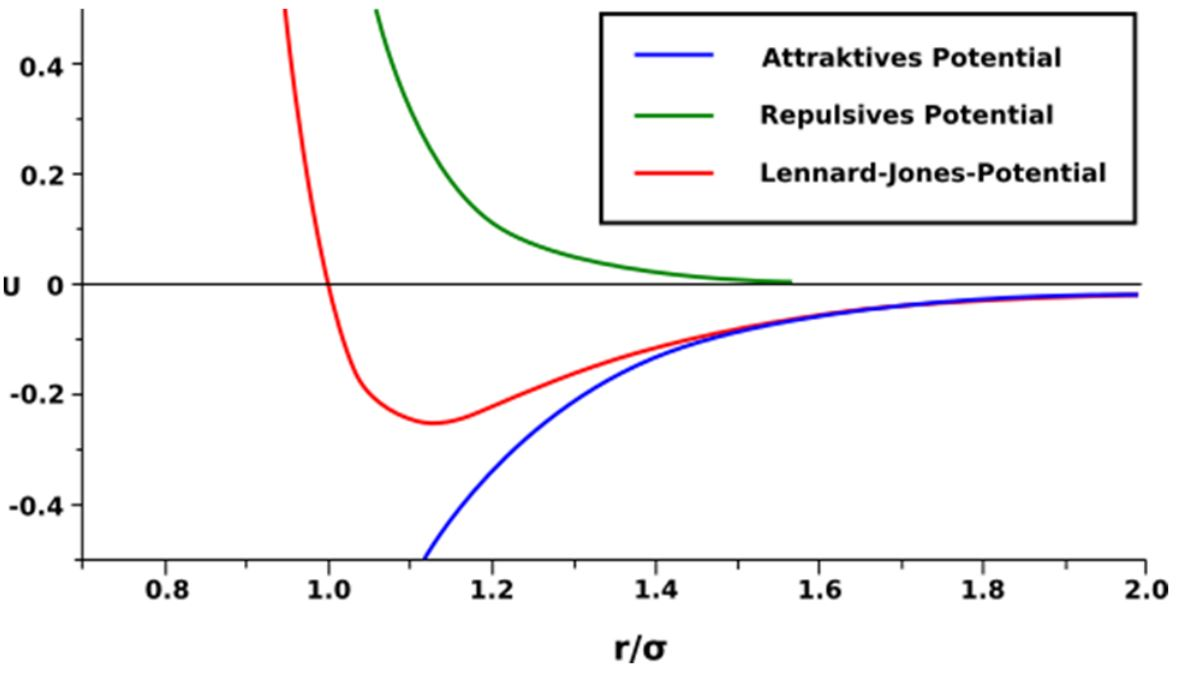
\includegraphics[width=0.8\textwidth]{content/plots/LJ.jpg}
  \caption{Leonard-Jones Potential zur Beschreibung der Wechselwirkung von Spitze und Probe nach \cite{Voigt}.}
  \label{fig:LJ}
\end{figure}
\subsection{Der Piezoelektrische-Effekt}
Der Piezoelektrische Effekt tritt nur bei Kristallen auf, die nicht centrosymmetrisch sind, beziehungsweise kein Inversionszentrum besitzen. Der Effekt beruht auf der Ausrichtung der im Festkörper vorhandenen elektrischen Dipole in einem externen elektrischen Feld. Das Feld sorgt für eine Verspannung des Kristalls in Form einer Ausdehnung des Materials.\\
Umgekehrt induziert die Verspannung eines Kristalls eine Ladung an der Oberfläche des Kristalls, wodurch ein elektrisches Feld endsteht. Dies wird auch als umgekehrter piezoelektrischer Effekt bezeichnet.\\
Da die Ausdehnung des Materials sehr gering ist, eignen sich piezoelektrische Materialien besonders, um die genaue Positionierung einer Untersuchten Probe im AFM zu Kontrollieren. Die Position der Probe kann dabei auf einige Nanometer genau kontrolliert werden.
\begin{SCfigure}
  \centering
  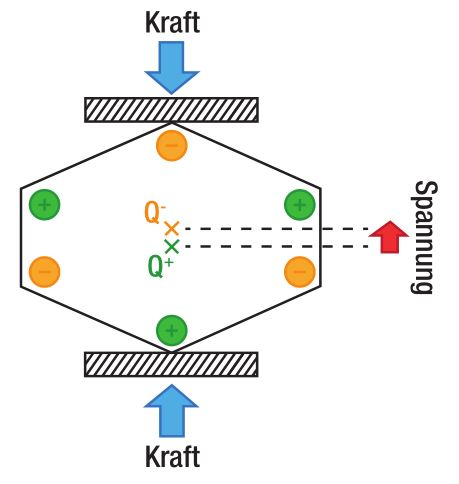
\includegraphics[width=0.5\textwidth]{content/plots/Piezo.jpg}
  \caption{Schemazeichnung des Piezoelektrischen Effekts. Durch Ausübung einer externen Kraft verschieben sich die vorhandenen Ladungen so, dass ein Ungleichgewicht entsteht, woraus eine elektrische Spannung resultiert.\cite{Thorlabs}}
  \label{fig:piezo}
\end{SCfigure}
%
\section{Experimentelle Grundlagen}
\subsection{Funktionsweise des AFM}
\label{subsec:afmfunk}
In der Rasterkraftmikroskopie wird die zu untersuchende Probe mittels einer Spitze abgerastert, welche an einem Balken (Englisch Cantilever) befestigt ist, welcher, je nach Kraft die auf die Spitze wirkt, ausgelenkt wird.
Damit das Mikroskop sensitiv für geringe Kraftunterschiede ist, muss der Cantilever eine geringe Federkonstante besitzen um kleine Auslenkungen detektieren zu können. Um die Auslenkung des Cantilevers detektieren zu können wird im vorliegenden Versuch das sogenannte Lichtzeigerprinzip verwendet. Dazu wird ein Fasergekoppelter Laser auf die Rückseite des Cantilevers fokussiert. Die Auslenkung des Cantilevers resultiert nun in einer räumlichen Verschiebung des reflektierten Laserstrahls. Diese Verschiebung kann mit einer Viersegment-Photodiode detektiert werden. Weitere Detektionsverfahren basieren z.B. auf interferometrischen, oder piezoresistiven Messungen der Auslenkung, sollen hier aber nicht genauer erläutert werden.\\
\\
Um die Probe abzurastern, wird nicht der Cantilever, sondern die Probe selbst verschoben. Dazu wird die Probe auf einer piezo-gesteuerten Positioniereinheit gelagert, sodass die Probe in $x-$ und $y-$ Richtung verschoben werden kann. Je nach Messmodus wird die Positioniereinheit außerdem dazu verwendet, den Abstand zwischen Probe und Spitze zu kontrollieren. Eine Schemazeichnung des verwendeten Rasterkraftmikroskop ist in \autoref{fig:Aufbauschema} dargestellt.
\begin{figure}[H]
\centering
  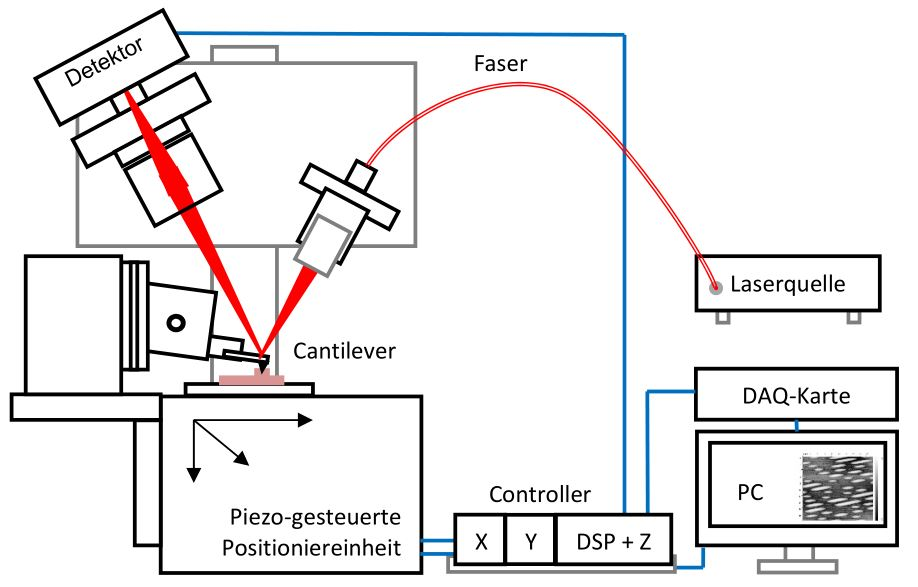
\includegraphics[width=\textwidth]{content/plots/Aufbau.jpg}
  \caption{Schema des Messaufbaus für ein Rasterkraftmikroskop.}
  \label{fig:Aufbauschema}
\end{figure}
Um die Höhe der Probe in Abhängigkeit vom gemessenen Signal kontrollieren zu können, wird die der Controller der Positioniereinheit mit der Photodiode verbunden. Die gemessenen Signale werden mithilfe einer DAQ-Karte ausgelesen und zur Weiterverarbeitung an einen Computer weitergeleitet.

\subsection{Messmodi}
\label{subsec:messmodi}
Um Scanlinien mit dem Rasterkraftmikroskop aufzunehmen gibt es mehrere mögliche Messmodi, in denen das Mikroskop betrieben werden kann. Dabei wird zwischen dynamischen und statischen Modi unterschieden.\\
Die statischen Messmodi finden Anwendung im, in \autoref{fig:Regime} gezeigten, Kontaktregime des AFM. Spitze und Probe sind in diesem Abstandsbereich in mechanischem Kontakt. Es ist nun möglich Messungen bei konstantem Abstand (\textit{constant-height-mode}) durchzuführen und die variierende Kraft als Messsignal zu wählen, oder die wirkende Kraft konstant zu halten (\textit{constant-force-mode}) und die variierende Höhe in Form eines Piezosignals zu Messen.\\
\begin{figure}[H]
  \centering
  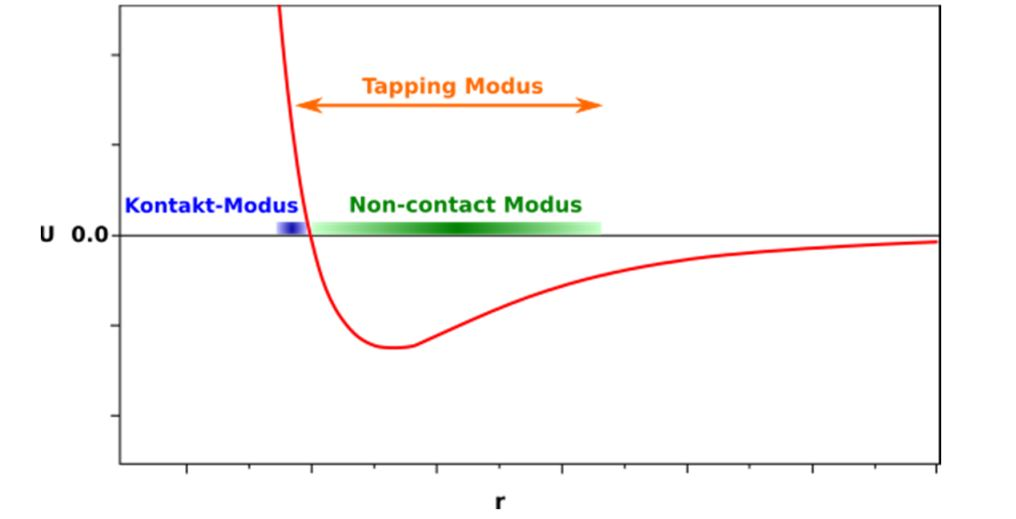
\includegraphics[width=\textwidth]{content/plots/regime.jpg}
  \caption{Unterscheidung der Messmodi je nach Potentialbereich, in denen die Messungen durchgeführt werden. Die Nullstelle des Potentials bildet die Grenze zwischen \textit{contact-} und \textit{non-contact mode}. Der \textit{tapping-mode} hat keinen festen Messbereich, da er ein dynamischer Messmodus ist. }
  \label{fig:Regime}
\end{figure}
Ein Nachteil der Messung bei konstanter Höhe ist das Risiko, die Spitze bei zu starken Kräften abzubrechen. Dies ist vor allem bei sehr unebenen Proben ein nicht zu vernachlässigendes Problem.
In diesem Experiment, werden daher alle Scans im \textit{constant-force-mode} durchgeführt. Um die zwischen Probe und Spitze wirkende Kraft konstant zu halten, wird das Auslenkungssignal von der Photodiode direkt an die Piezo-Positioniereinheit zurückgegeben, sodass die Höhe der Einheit präzise und schnell nachgeregelt wird.\\
\\
Im dynamischen Messbetrieb wird der Cantilever, beispielsweise durch eine zweite Piezoschaltung, extern in Schwingungen versetzt. Dies kann wahlweise direkt (\textit{dynamic mode}), oder nah an (\textit{intermitting mode} oder \textit{tapping mode}) Resonanzfrequenz geschehen. Verändert sich nun die zwischen Probe und Spitze wirkende Kraft, so kommt es zu einer Änderung der Resonanzfrequenz. Je nach Messmodus kann nun die Frequenzverschiebung, oder die Amplitude der Schwingung als zur Kraft korrespondierende Messgröße verwendet werden. Messungen im \textit{dynamic-mode} werden ohne durchgehenden direkten mechanischen Kontakt und üblicherweise im Vakuum bzw. Hochvakuum durchgeführt. Mithilfe des \textit{intermitting-mode} sind auch Messungen bei Normalbedingungen und in Flüssigkeiten möglich.
Messungen im dynamischen Modus bieten im allgemeinen zwar bessere Auflösungen als statische, sind dafür aber zeitaufwendiger.

\subsection{Scanlinien und Scanartefakte}
Die beim Abrastern der Probe entstehenden Scanlinien beschreiben das Höhenprofil der Oberfläche der Probe. Dabei ist darauf zu achten, dass die aufgenommene Scanlinie der Faltung der Probenoberfläche mit der verwendeten Spitze entspricht. \footnote{Es handelt sich hier um die Faltungen der Funktionen, mit denen Oberfläche und Spitze moduliert werden.} Unebenheiten an der Spitze gehen also ebenfalls in das gemessene Signal mit ein und verunreinigen die eigentliche Scanlinie. Um unebenheiten auf der Spitze festzustellen, können bekannte Proben mit möglichst scharfen Kanten vermessen werden. Mithilfe von Proben, deren Oberfläche selbst sehr Scharfe Spitzen beinhaltet, lässt sich auch umgekehrt eine Scanlinie der Rasterspitze selbst aufnehmen.\\
\\
Ein weiteres Scanartefakt, welches maßgeblichen Einfluss auf die Genauigkeit der Scanlinien hat, ist die Hysterese der Piezoelemente. Die Ausdehnung und das Zusammenschrumpfen der Piezoelemente ist ein nicht exakt linearer Prozess. Die Hysterese der Piezomaterialien sorgt nun dafür, dass sich das Material nicht exakt genauso ausdehnt, wie es sich zusammenzieht. Der Vorgang ist in \autoref{fig:hysterese} dargestellt.
\begin{figure}[H]
  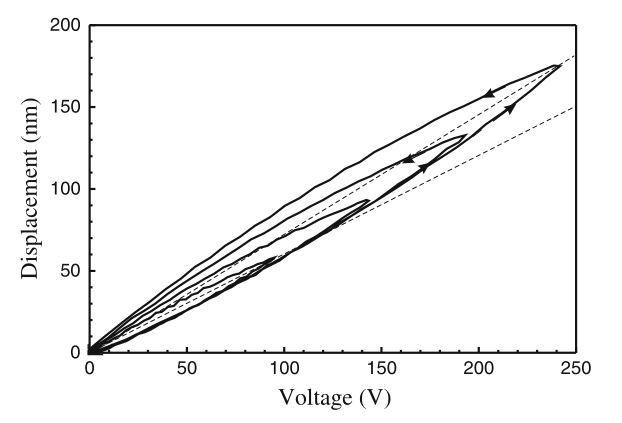
\includegraphics[width=0.7\textwidth]{content/plots/hysterese.jpg}
  \caption{Hysteresekurve eines Piezokristalls, im für Rasterkraftmikroskopie relevanten Bereich. \cite{Voigt}}
  \label{fig:hysterese}
\end{figure}
Mithilfe der sogenannten \textit{strain-gauge-method} ist es möglich den Einfluss der Hysterese zu vermindern. Dazu werden Dehnungsmesstreifen auf die Piezoelemente aufgeklebt, welche die Ausdehnung und das Zusammenziehen präzise Messen können, sodass die enstehenden Fehler beim Auswerten der Scanlinien berücksichtigt werden können.\\
\\
Da die Änderungen der Ladungsverteilung in den Piezoelementen nicht instantan vonstatten geht ist das AFM in seiner Auflösung ebenfalls beschränkt. Bei sehr schnell variierenden Messsignalen kommt es dadurch zu einer Verzögerung aufgrund der länger dauernden Ausrichtung der Dipole im Material. Dieses Scanartefakt wird auch als \textit{creep} bezeichnet.
\\
Ebenfalls zu berücksichtigen sind thermale Drifts in allen mechanischen Komponenten des Systems. Wird nicht im UHV gemessen ist es außerdem möglich, dass sich auf der Probenoberfläche ein Wasserfilm bildet. Dadurch bildet sich bei heranfahren der Spitze an die Oberfläche ein Wassermeniskus, in dem anziehende Kapillarkräfte wirken. Dies nimmt ebenfalls Einfluss auf die in \autoref{sec:KAK} erläuterten Messungen von Kraft-Abstands Kurven.\\
\newpage
\subsection{Kraft-Abstands-Kurven}
\label{sec:KAK}
Neben der Analyse der Oberflächenstruktur, lassen sich mit einem Rasterkraftmikroskop auch gezielt mechanische Eigenschaften der Materialoberfläche untersuchen. Dies gelingt durch Messungen von Kraft-Abstands-Kurven. Die Spitze des AFM wird dabei in die Probe hinein gedrückt und wieder heraus gezogen. So lässt sich die Kraft als Funktion des Abstandes zwischen Probe und Spitze aufnehmen.
In \autoref{fig:KAK} sind Typische Kraft-Abstands-Kurven für ein weiches und ein hartes Material dargestellt. Die blaue Kurve beschreibt dabei das Eindrücken der Probe und die rote das Herausziehen der Spitze aus der Probe.
\begin{figure}[H]
  \centering
  \label{fig:KAK}
  \begin{subfigure}{0.45\textwidth}
    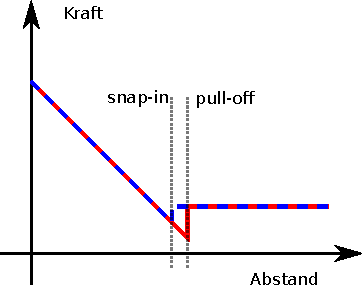
\includegraphics{content/plots/harte-theorie.pdf}
    \caption{Harte Probe.}
  \end{subfigure}
  \begin{subfigure}{0.45\textwidth}
    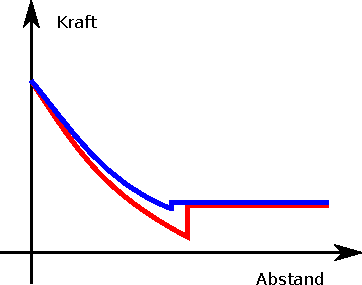
\includegraphics{content/plots/weiche-theorie.pdf}
    \caption{Weiche Probe.}
  \end{subfigure}
  \caption{Schema von Kraft-Abstands-Kurven für Proben unterschiedlicher Härte.}
\end{figure}
Beim heranfahren an die Oberfläche wird für einen bestimmten Abstand eine schlagartige Änderung der Kraft detektiert, die durch das Einsetzen der kurzreichweitigen Wechselwirkungen zustande kommt (\textit{snap-in}). Auf dem Rückweg der Spitze entsteht durch die wirkende Adhäsionskraft ein sogenannter \textit{pull-off}. Mithilfe dieser Effekte kann die Adhäsionskraft in \autoref{sec:bla?} bestimmt werden.
Um aus der Kraft-Abstands-Kurve den Elastizitätsmodul der untersuchten Probe zu bestimmen, muss zunächst die Federkonstante des Cantilevers ermittelt werden. Diese kann mithilfe der Formel
\begin{equation}
  \label{eqn:federkonst}
  k = \frac{E_c\cdot w\cdot t^3}{4\cdot l}
\end{equation}
aus Breite $w$, Höhe $t$ und Länge $l$ des Cantilevers berechnet werden. Außerdem geht der Elastizitätsmodul $E_c$ des Cantilevermaterials in die Berechnung ein.\\
\\
Aus der von I. Sneddon erweiterten Hertzschen Modell der Kontaktmechanik lässt sich nun eine Formel für den Elastizitätsmodul der Oberfläche der Probe ableiten. Das Modell beschreibt das Eindrücken eines Stempels in einen elastischen Halbraum. Der Stempel entsprichnt beim AFM der Spitze am Cantilever und wird durch einen Kegel modelliert. Für die Kraft $F$ zwischen Spitze und Probe ergibt sich so die Formel
\begin{equation}
  \label{eqn:emodul}
  F = \frac{2}{\pi} \tan{(\alpha)}\cdot\frac{E}{1-\nu^2}\cdot\delta^2\, .
\end{equation}
Dabei ist $\nu$ die Poissonzahl und $\delta$ die Verformung der Oberfläche.
Die Kegelgeometrie geht dabei in Form des halben Öffnungswinkel $\alpha$ in die Formel ein.
bestimmung emodul , adhäsionskräfte
contact regime ljp
snap in pull of
hart weich
federkonstante
